\documentclass{standalone}
\usepackage{tikz}
\usetikzlibrary{backgrounds}
\begin{document}
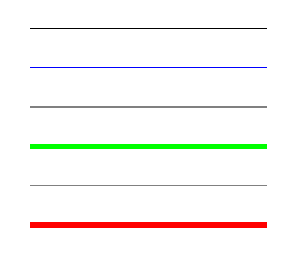
\begin{tikzpicture}
  \begin{scope}[line width=2pt]
    \draw[red] (0,0) -- (3,0);
    \begin{scope}[on background layer]
      \draw[gray] (0,0.5) -- (3,0.5);
    \end{scope}
    % Still 2pt: the key entered the layer inside its own scope.
    \draw[green] (0,1) -- (3,1);
    \begin{pgfonlayer}{background}
      \draw[gray] (0,1.5) -- (3,1.5);
    \end{pgfonlayer}
    % 0.4pt: \pgfonlayer set the line width in this scope before opening the layer.
    \draw[blue] (0,2) -- (3,2);
  \end{scope}
  \draw[black] (0,2.5) -- (3,2.5);
\end{tikzpicture}
\end{document}
